\PassOptionsToPackage{unicode=true}{hyperref} % options for packages loaded elsewhere
\PassOptionsToPackage{hyphens}{url}
%
\documentclass[english,]{article}
\usepackage{lmodern}
\usepackage{amssymb,amsmath}
\usepackage{ifxetex,ifluatex}
\usepackage{fixltx2e} % provides \textsubscript
\ifnum 0\ifxetex 1\fi\ifluatex 1\fi=0 % if pdftex
  \usepackage[T1]{fontenc}
  \usepackage[utf8]{inputenc}
  \usepackage{textcomp} % provides euro and other symbols
\else % if luatex or xelatex
  \usepackage{unicode-math}
  \defaultfontfeatures{Ligatures=TeX,Scale=MatchLowercase}
\fi
% use upquote if available, for straight quotes in verbatim environments
\IfFileExists{upquote.sty}{\usepackage{upquote}}{}
% use microtype if available
\IfFileExists{microtype.sty}{%
\usepackage[]{microtype}
\UseMicrotypeSet[protrusion]{basicmath} % disable protrusion for tt fonts
}{}
\IfFileExists{parskip.sty}{%
\usepackage{parskip}
}{% else
\setlength{\parindent}{0pt}
\setlength{\parskip}{6pt plus 2pt minus 1pt}
}
\usepackage{hyperref}
\hypersetup{
            pdftitle={My Resume},
            pdfborder={0 0 0},
            breaklinks=true}
\urlstyle{same}  % don't use monospace font for urls
\usepackage{graphicx,grffile}
\makeatletter
\def\maxwidth{\ifdim\Gin@nat@width>\linewidth\linewidth\else\Gin@nat@width\fi}
\def\maxheight{\ifdim\Gin@nat@height>\textheight\textheight\else\Gin@nat@height\fi}
\makeatother
% Scale images if necessary, so that they will not overflow the page
% margins by default, and it is still possible to overwrite the defaults
% using explicit options in \includegraphics[width, height, ...]{}
\setkeys{Gin}{width=\maxwidth,height=\maxheight,keepaspectratio}
\setlength{\emergencystretch}{3em}  % prevent overfull lines
\providecommand{\tightlist}{%
  \setlength{\itemsep}{0pt}\setlength{\parskip}{0pt}}
\setcounter{secnumdepth}{0}
% Redefines (sub)paragraphs to behave more like sections
\ifx\paragraph\undefined\else
\let\oldparagraph\paragraph
\renewcommand{\paragraph}[1]{\oldparagraph{#1}\mbox{}}
\fi
\ifx\subparagraph\undefined\else
\let\oldsubparagraph\subparagraph
\renewcommand{\subparagraph}[1]{\oldsubparagraph{#1}\mbox{}}
\fi

% set default figure placement to htbp
\makeatletter
\def\fps@figure{htbp}
\makeatother

\ifnum 0\ifxetex 1\fi\ifluatex 1\fi=0 % if pdftex
  \usepackage[shorthands=off,main=english]{babel}
\else
  % load polyglossia as late as possible as it *could* call bidi if RTL lang (e.g. Hebrew or Arabic)
  \usepackage{polyglossia}
  \setmainlanguage[]{english}
\fi

\title{My Resume}
\date{}

\begin{document}
\maketitle

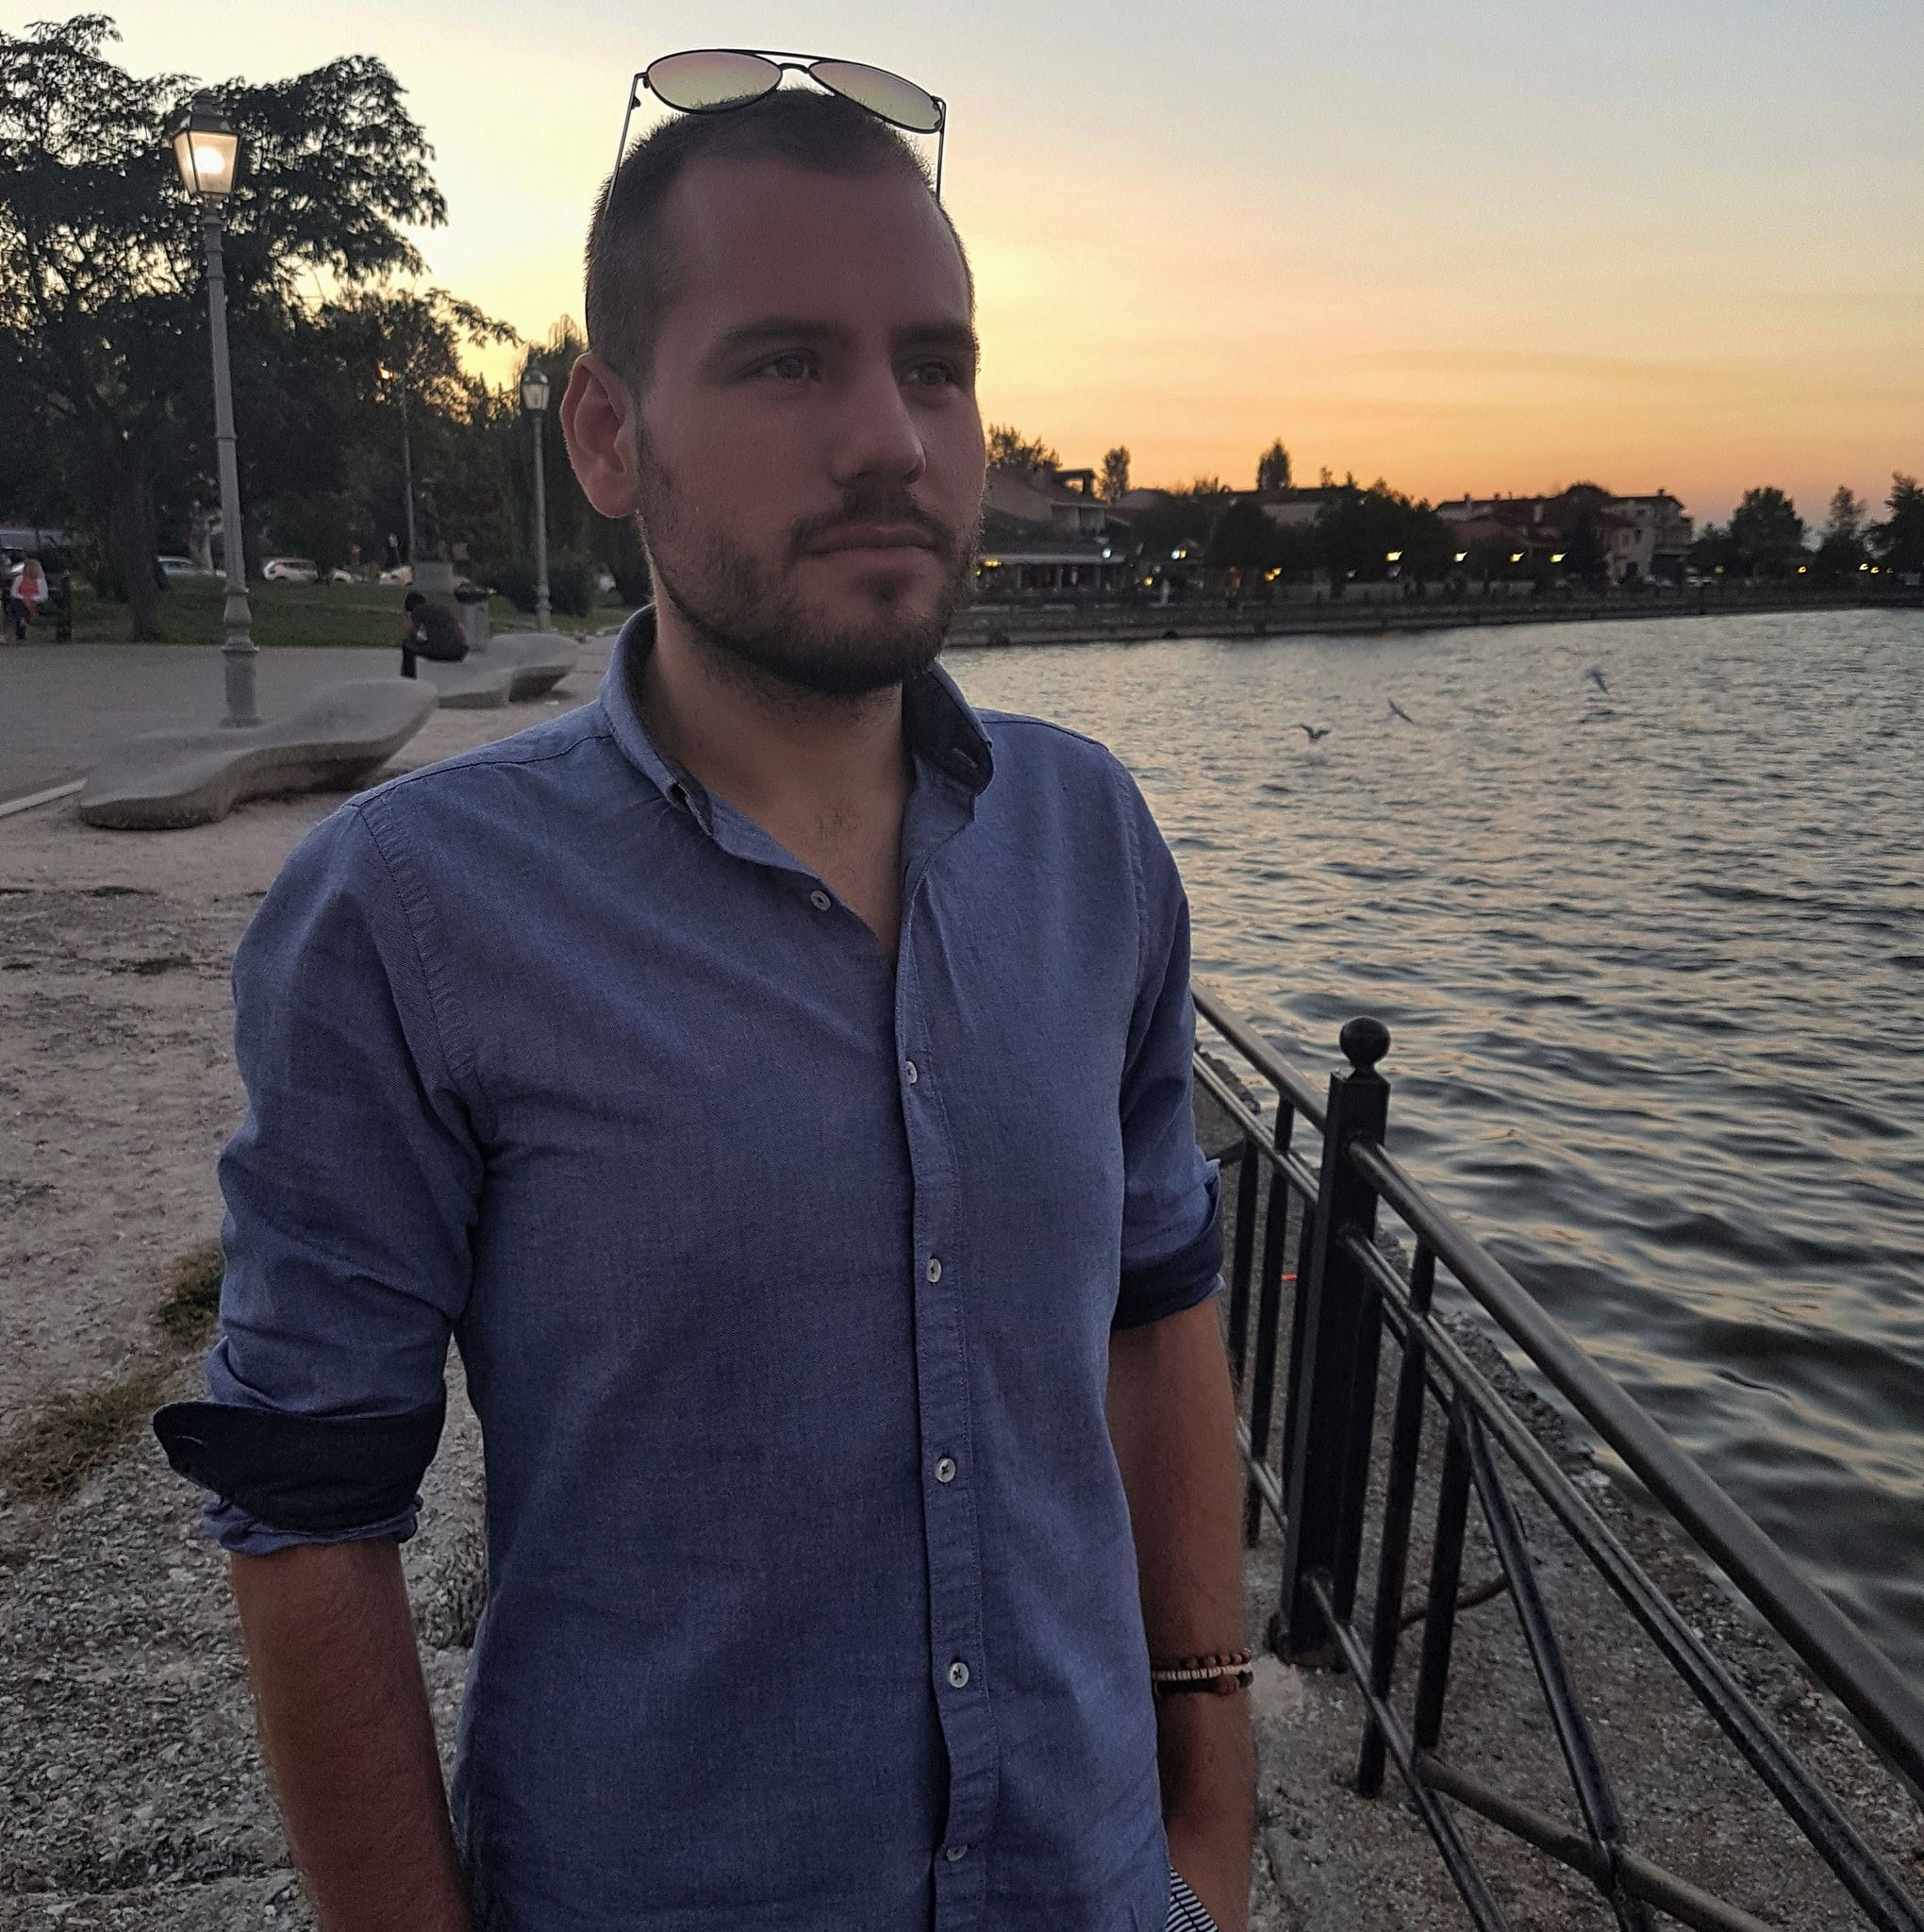
\includegraphics{/online-cv/assets/images/profile.png}

\hypertarget{george-palantzas}{%
\section{George Palantzas}\label{george-palantzas}}

\hypertarget{developer}{%
\subsubsection{Developer}\label{developer}}

\begin{itemize}
\tightlist
\item
  \emph{}
  \href{mailto:palantzasgeorge@yahoo.gr}{\nolinkurl{palantzasgeorge@yahoo.gr}}
\item
  \emph{} \href{tel:6972638127}{6972638127}
\item
  \emph{} \href{http://github.com/geopala}{github.com/geopala}
\item
  \emph{} \href{https://linkedin.com/in/geopala}{geopala}
\item
  \emph{} \href{http://github.com/geopala}{geopala}
\item
  \emph{} \href{https://twitter.com/@geopala}{@geopala}
\end{itemize}

\hypertarget{education}{%
\subsection{Education}\label{education}}

\hypertarget{bsc-in-computer-science}{%
\paragraph{BSc in Computer Science}\label{bsc-in-computer-science}}

\hypertarget{ionian-university}{%
\subparagraph{Ionian University}\label{ionian-university}}

2007 - 2021

\hypertarget{languages}{%
\subsection{Languages}\label{languages}}

\begin{itemize}
\tightlist
\item
  Greek {(Native)}
\item
  English {(Professional)}
\end{itemize}

\hypertarget{interests}{%
\subsection{Interests}\label{interests}}

\begin{itemize}
\tightlist
\item
  Coding
\item
  Traveling
\end{itemize}

\hypertarget{about-theme}{%
\subsection{About Theme}\label{about-theme}}

\begin{itemize}
\tightlist
\item
  \href{https://www.youtube.com/watch?v=Jnmj1dXDbNk}{How to use?}
\item
  \href{https://github.com/sharu725/online-cv}{Star}
\end{itemize}

\hypertarget{career-profile}{%
\subsection{\texorpdfstring{{ \emph{} \emph{} } Career
Profile}{    Career Profile}}\label{career-profile}}

Undergraduate student at Ionian University

\hypertarget{experiences}{%
\subsection{\texorpdfstring{{ \emph{} \emph{} }
Experiences}{    Experiences}}\label{experiences}}

\hypertarget{bsc-in-computer-science-1}{%
\subsubsection{BSc in Computer
Science}\label{bsc-in-computer-science-1}}

2007 - 2021

Ionian University

The graduate of the Department of Informatics has the scientific and
technical expertise to work as an IT professional, either as
self-employed, or as an executive in the private or public sector. More
specifically he can be employed as:

\begin{itemize}
\tightlist
\item
  Software Engineer
\item
  Computer Systems Engineer
\item
  Network and Telecommunications Engineer / Administrator
\item
  Database Administrator
\end{itemize}

\hypertarget{projects}{%
\subsection{\texorpdfstring{{ \emph{} \emph{} }
Projects}{    Projects}}\label{projects}}

{ \protect\hyperlink{hook}{OpenValue} } - {Measuring the value of
official municipal open data in a smart city.}

\hypertarget{publications}{%
\subsection{\texorpdfstring{{ \emph{} \emph{} }
Publications}{    Publications}}\label{publications}}

\protect\hyperlink{}{Planning a smart city's strategy and the value of
open data}

George Palantzas

Ionian University, 2021

\hypertarget{skills-proficiency}{%
\subsection{\texorpdfstring{{ \emph{} \emph{} } Skills \&
Proficiency}{    Skills \& Proficiency}}\label{skills-proficiency}}

\hypertarget{python-django}{%
\subsubsection{Python \& Django}\label{python-django}}

\hypertarget{javascript-jquery}{%
\subsubsection{Javascript \& jQuery}\label{javascript-jquery}}

\hypertarget{html5-css}{%
\subsubsection{HTML5 \& CSS}\label{html5-css}}

\hypertarget{ruby-on-rails}{%
\subsubsection{Ruby on Rails}\label{ruby-on-rails}}

\hypertarget{sketch-photoshop}{%
\subsubsection{Sketch \& Photoshop}\label{sketch-photoshop}}

{Designed with \emph{} by \href{http://themes.3rdwavemedia.com}{Xiaoying
Riley}}

\end{document}
